\chapter{Design}
This chapter aims to introduce and discuss various aspects of the design process for the semantic mashup and the working of the focused scraper. In particular, the first section will provide some background context on website scraping. Then, the detailed design of the semantic mashup and the focused scraper program will be introduced. Then, an account is following on how the focused scraper can be managed in the mashup application.

\section{Scraping techniques}
Web scraping is the technique of automated information extraction from one or more web sites. Web scraping uses many strategies, to achieve this goal. The ones used for this thesis are described below.

\subsection{Using regular expressions}
One strategy for web scraping is that of, using regular expressions to analyze the source code of the target web page. A regular expression is a piece of string that describes the structure of a larger text. Since all web pages are made out of text, excluding images and videos, regular expressions are effective. With the help of regular expressions, bits and pieces of the page can be examined in isolation. For example, “<p>.+?</p>” will match a paragraph of text. Although regular expressions are useful, they can not be used to parse HTML fully, because HTML has too many rules and exceptions. To parse HTML fully, we need a HTML parser or a DOM parser.

\subsection{Using DOM parsing}
An HTML document once parsed, becomes a DOM object, in the browser. On a DOM object, a number of useful operations like, selecting all headings, selecting particular section, selecting a particular class of paragraph elements can be performed. There exist many libraries in Python that simulate the browser and create a DOM object. We have used Beautiful Soup 4 \cite{6}.

\subsection{Web Robot Programming}
A web robot simulates the actions of a user in a browser window. For example, if the user
\begin{enumerate}
\item Opened a browser
\item Typed www.google.com in the URL bar
\item Pressed 'Enter'
\item Entered a query “restaurants in Liverpool”
\item Pressed “Go”
\item Clicked on the first result
\end{enumerate}

The user is displayed the first result's web page. In this case, namely \\
\emph{http://www.gustorestaurants.uk.com/restaurants/gusto-liverpool}. All these actions can be simulated programatically with the help of a Web Robot, often shortened to as a bot program.

As it can easily be imagined, using a bot one can simulate many actions on a website and one can extract useful information after an interaction with it, virtually. Interactivity with the web page in question is the key feature that differentiates crawling from scraping. Python provides an excellent library, specialized for bot programming, which we have used.

\section{Content Sources}
The content sources of our mashup are the following three: \emph{restaurant-guide.com}, Google maps and \emph{ratings.food.gov.uk}. The first website provides restaurant details like cuisine, address, opening/closing timings, phone. Google maps provides us with a map pointing to the restaurant location. And finally the latter provides food hygiene ratings from the Food Standards Agency of UK.
Below the first of the sources is displayed.

\begin{figure}[!htb]
  \centering
  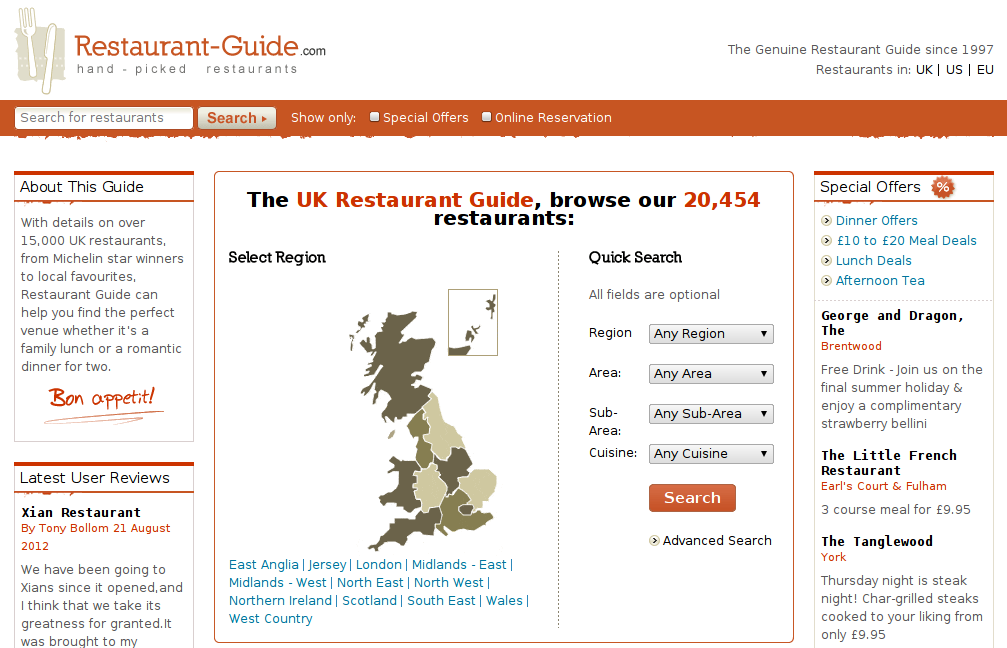
\includegraphics[width=16cm]{fig/restaurant_guide.png}
  \caption[ http://restaurant-guide.com]
  {shows our content source restaurant-guide.com}
\end{figure}

\begin{figure}[!htb]
  \centering
  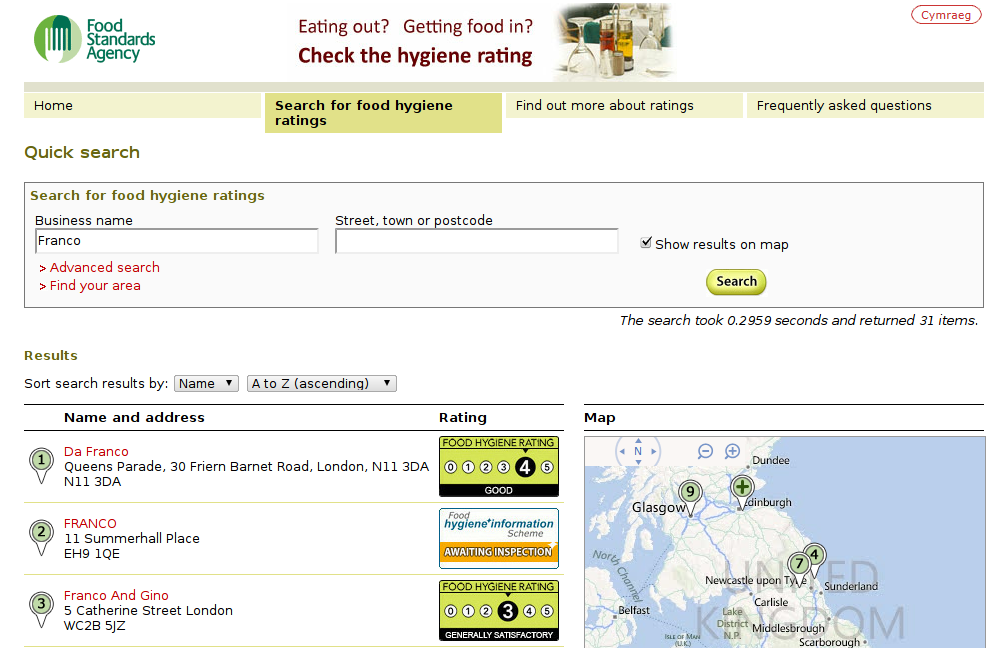
\includegraphics[width=16cm]{fig/fsa_ratings.png}
  \caption[ http://ratings.food.gov.uk]
  {shows another content source ratings.food.gov.uk}
\end{figure}


\section{Mashup User Interface}

We have given our designed application, a simple name: we call it 'RestaurantGO'. For the mashup to work, the user just has to type the cuisine name and run the search. For instance, 'Italian Coventry'. It will provide results of a list of restaurants with predefined semantic annotations.

\begin{figure}[!h]
  \centering
  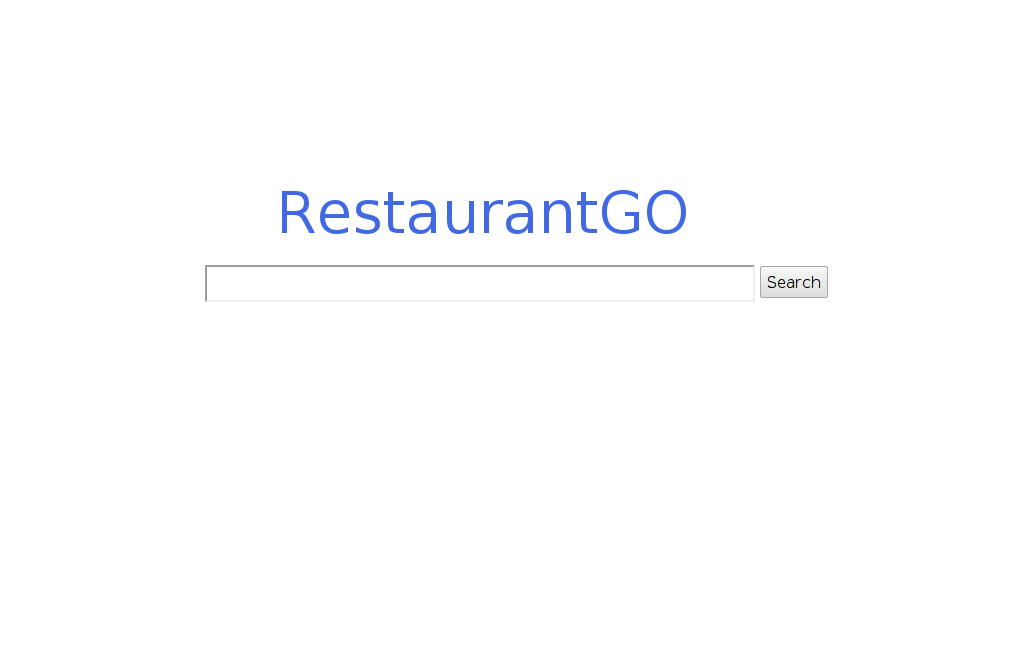
\includegraphics[width=16cm]{fig/restaurant_go.png}
  \caption[ RestaurantGo home page]
  {shows home page of our mashup RestaurantGo}
  \label{fig: 3.3}
\end{figure}

The results were obtained by scraping the source website restaurant-guide.com which searches for Italian restaurants and gathers the data for every restaurant record. These attributes for every restaurant are categorized under our custom designed columns such as address, type of cuisine, phone, opening times, lunch and dinner prices. Google maps location based information was also obtained. In the next section, we move onto the working of our mashup.

\newpage
\begin{figure}[!h]
  \centering
  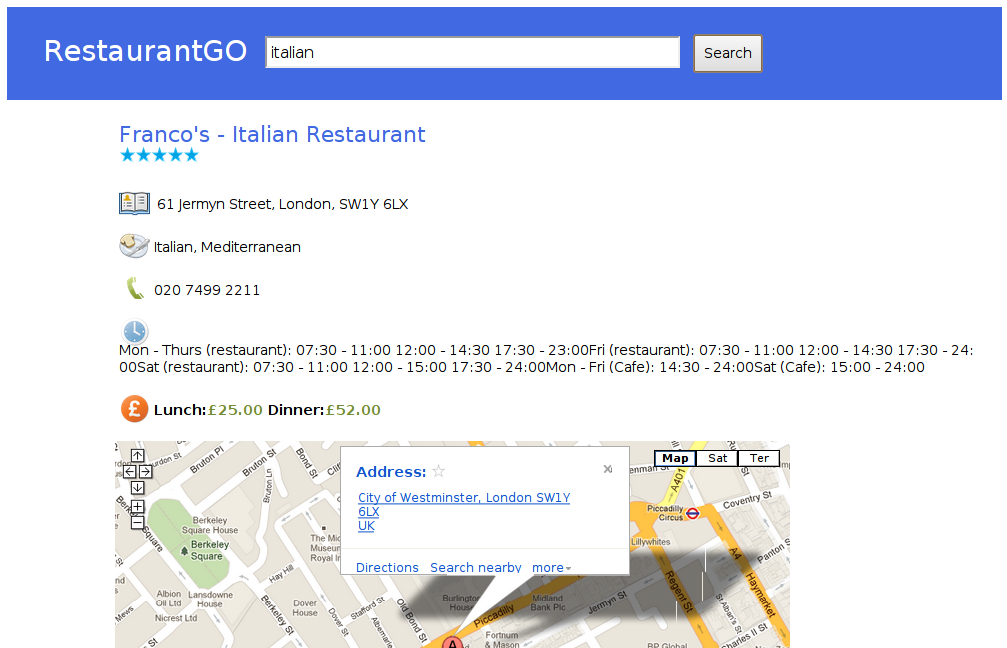
\includegraphics[width=16cm]{fig/restaurant_go_results.png}
  \caption[ RestaurantGo search results]
  {shows RestaurantGo's search results for Italian cuisine}
  \label{fig: 3.4}
\end{figure}

\section{Scraping program}
Our program involves running a local server on a client browser. In order to accomplish this, we have to install certain Python libraries. They are:
\begin{enumerate}
\item \textsl{Flask:} This is a small framework in Python which has a built-in development server \cite{24}. This was considered suitable for our project. Its methods were used to run our GET method and render custom designed html files.
\item \textsl{BeautifulSoup:} It’s a Python library useful for extracting data from HTML and XML files \cite{6}. It works along with an html parser and has many objects suited to working with html tags in scraping data.
\item \textsl{mechanize:} This is another another library useful for web programming in Python. The main feature is that we can emulate a browser and task automation \cite{5}.
\item Other standard packages \textbf{sqllite 3, re, json, urllib}, are all available in Python 2.7. \textsl{SQLite} is used for storing the results obtained. \textsl{urllib} is used for parsing the related web pages via their URLs. \textsl{json} is an object notation library for presenting results via a suitable format.
\end{enumerate}

\subsection{Architecture}
To get an overview of the application created in this research thesis, RrestaurantGo, it is important to understand the architectural principles involved in building it. RestaurantGo is first and foremost a Flask Web Application. Flask framework internally follows the REST paradigm. REST is a predominant web service design model. It utilizes the HTTP protocol verbs “GET”, “POST”, “PUT”, “DELETE” and others to build web services on top of it. Once the Flask Web Application server (HTTP Server) is started, each and every Form submitted, and the URL entered in the URL bar or clicked on the page, maps to a REST call like “GET /url”. These calls are called “routes” by the Flask framework. Each route has a handler which gets executed and serves the particular web page or a web resource. The user interacts with the web resource and produces more REST calls as a result of his actions. And in this way the user-application interaction cycle continues, till the the user reaches his goal.

\begin{figure}[!htb]
  \centering
  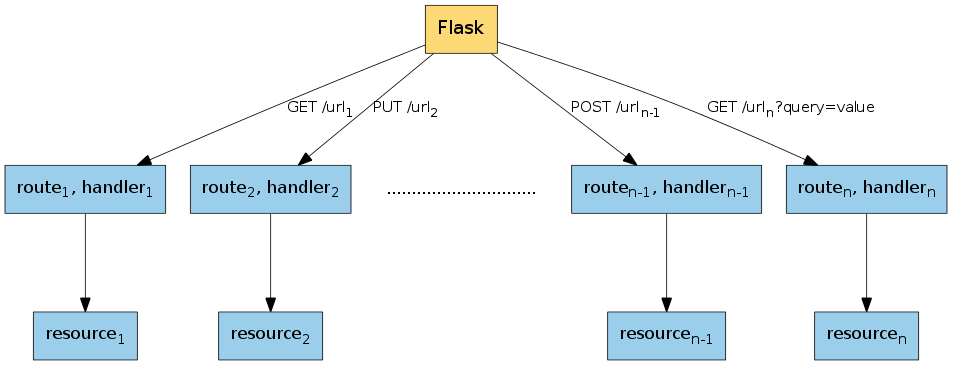
\includegraphics[width=16cm]{fig/flask.png}
  \caption[Workflow of a Flask application]
  {shows workflow of request and routes in a Flask application}
\end{figure}

The above figure shows how the Flask framework, in general serves web requests. Once the Flask HTTP server starts, it listens to various HTTP requests like “GET”, “PUT”, “POST” initiated by the user. For each request a handler gets executed which serves the results. In the context of our mashup application, see Figure ~\ref{fig: 3.6}.

\begin{figure}[!htb]
  \centering
  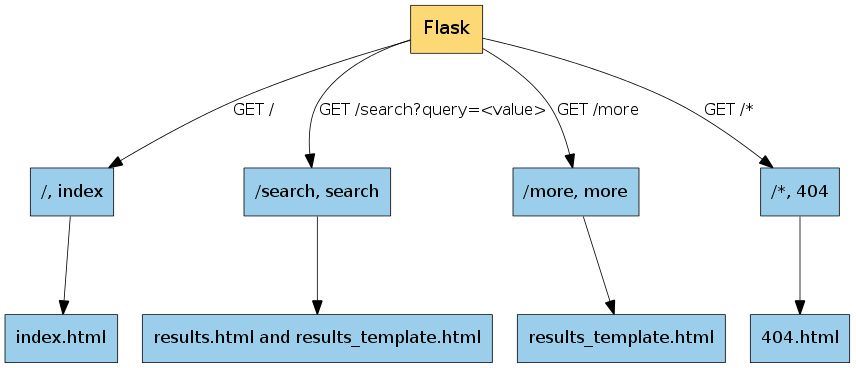
\includegraphics[width=16cm]{fig/rest.png}
  \caption[Workflow of RestaurantGo]
  {shows the REST workflow of Flask in RestaurantGo}
  \label{fig: 3.6}
\end{figure}



After starting the web server, when the user enters the url \emph{localhost:5000} in his browser, the user is immediately presented with the contents of index.html (Fig ~\ref{fig: 3.3}). This is because, “/” is considered as the route when only the url is given. Now from that page,the user can enter a query in the search form. Once the search button is clicked, the user is directed to the results.html page (Fig ~\ref{fig: 3.4}). Between the search request and the delivering of the results, the “search” handler gets executed. It is this handler that scrapes the content sources. Similarly when the user wants more results from the results page, he clicks ``More Results ...'' and this executes the more handler through the /more route, asynchronously using AJAX. The more handler returns more of the scraped results, which gets added to the already existing results by JavaScript. Finally, when the user enters a wrong URL, he is promptly showed the standard 404 Not Found web page.

The functionality of the mashup is delivered by the search and more handlers. Since both are similar in design, we will discuss the search handler below.

When the user enters a search query for “Liverpool”, the following micro-actions happen:
\begin{enumerate}
\item The browser sends a “GET  /search?query=Liverpool” to Flask
\item Flask deciphers the GET request and retrieves the corresponding route, here – “/search”
\item Flask starts the execution of the handler for “/search” route, which in this case is “search”.
\item Search handler stores “Liverpool” under the cookie name “query”. This will come in handy when the \textsl{more} handler gets executed. Because cookies are persisted across web requests, the more handler can know the query implicitly via the browser cookie.
\item The database is queried for “Liverpool”. If it is a hit, no further processing is required and one can directly jump to step 9.
\item If the Database query is a miss, then it means we have to scrape the results from the content sources. To do this a special helper class “RestaurantGuide” is called upon. The idea of using a special helper class is to isolate all the scraping logic of a content source into a separate module. Then, the search method of Restaurant Guide is called.
  
  
  
\item The scraping actions of the search method, performs the following:
  \begin{itemize}
  \item Creates a virtual browser object using mechanize.
  \item Open www.restaurant-guide.com in the virtual borswer
  \item Find the search form and submit “Liverpool” there.
  \item Wait for the result. The result is a HTML page.
  \item Pass on the result to BeatifulSoup DOM parser.
  \item Extract the restaurant data from restaurant-guide.com with the help of BeautifulSoup.
  \item Repeat the above process for ratings.food.gov.uk. Except this time, use regex for parsing.
  \item Return the extracted data to the search handler
  \end{itemize}
\item With the results in hand, the search handler now stores the results into the database for future use.
\item The results and a template “results.html” are taken and rendered to the user with the help of Flask's render\_template function. A template is a special html file. Since HTML is a declarative language, it does not support variables, if and while loops. A template consists of precisely these extra features. However, a browser cannot understand these features. Therefore a template has to be pre-processed to remove and evaluate the extra tokens. That is the job of render\_template.
  
\end{enumerate}
The flowchart of the workings of our mashup is given in the next page.

\begin{figure}[!htb]
  \centering
  \caption[Flowchart showing the working of  RestaurantGo]
  {shows the working of our Mashup -- RestaurantGo}
  \vspace{0.8cm}
  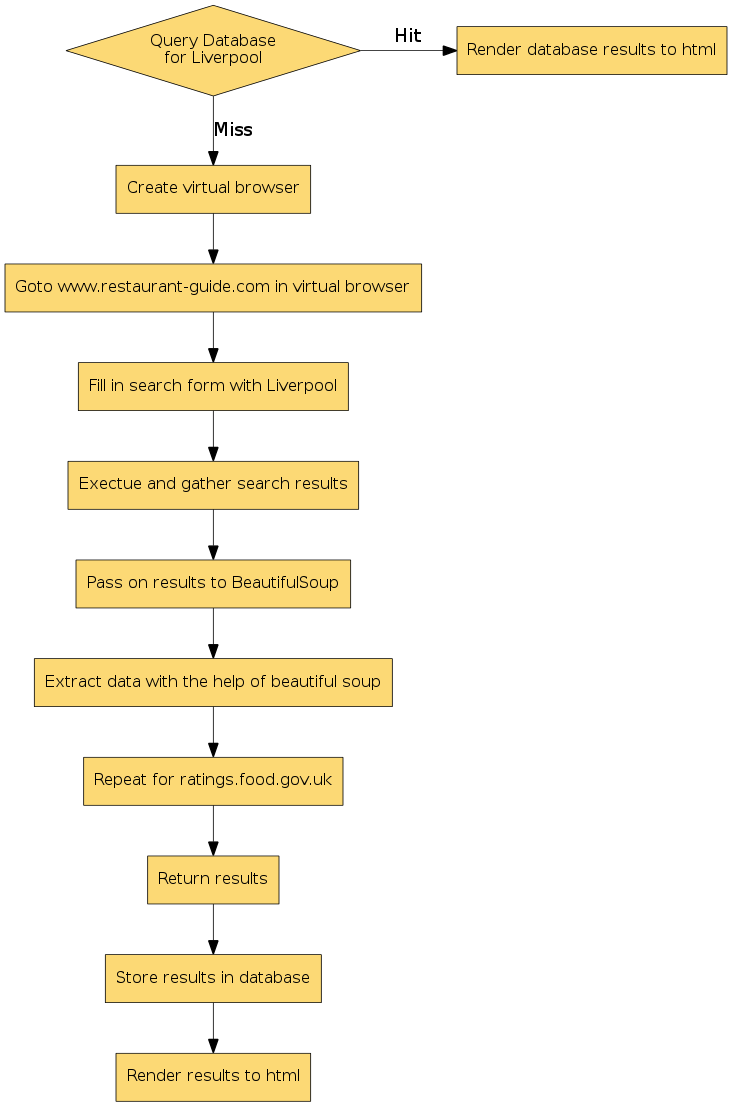
\includegraphics[width=16cm]{fig/flow_chart.png}
\end{figure}

